%Victor
\section{Suite de protocole}

\subsection{ARP}
ARP (Address resolution protocol) est un protocole à cheval entre la couche 2 et
la couche 3 permettant de faire la conversion entre les adresses de niveau 2 et de niveau 3.
Cela est très utilisé étant donné que les hôte connaissent souvent les adresses IP de leur destinataire,
mais rarement l'adresse de niveau 2 de ce destinataire ou de la passerelle à contacter pour joindre
le destinataire.

\subsubsection{Cache ARP}
Le cache ARP ou table ARP est une table sotcké en local par un hôte et qui ressence les associations entre adresse IP et adresse MAC.
Ces associations peuvent être soit de type statique, donc écrite "en dur" par l'administrateur, ou dynamique, donc issue d'échange de trame ARP,
et qui possèdent, en plus des associations statique, une durée de validité, étant donné qu'une interface peut changer d'adresse IP et qu'il vaut
maintenir la table à jour.
Cette table peut donc être représenté comme une suite d'entrés, contenant chacune une adresse IP, une adresse MAC et éventuellement une durée de vie.

\subsubsection{Entête}
//TODO


\subsubsection{Fonctionnement}
Prenons l'exemple où A veux envoyer un message à B. A connait l'adresse IP de
B. Donc A va préparer son paquet qu'il va envoyer à B, avec son adresse IP en
source et l'adresse IP de B en destination. La paquet passe dans la couche
liaison, il va être enpaqueté dans une trame de niveau 2. Cette trame aura
comme adresse source l'adresse de niveau 2 de A, mais à ce moment il ne peux
pas completé l'adresse destination de la trame: en effet, il ne connait
l'adresse de niveau 2 du destinataire. La paquet reste bloqué en couche 2 et ne
peux pas être envoyé au destinataire. Comment obtenir l'adresse de niveau 2 du destinaire?
Le protocole ARP est capable de faire cette translation.

Pour faire cela l'hôte A va tout d'abord regarder dans sa table ARP si il n'a pas une entrée pour l'adresse IP à laquelle il souhaite envoyer son paquet. Si il tourve une correpondance, il va utiliser l'adresse MAC stocker en correspondance avec l'adresse IP recherché.
Si il ne trouve pas de correspondance il va emmetre une trame ARPREQUEST pour tenter de contacter le possesseur de l'adresse IP qu'il souhaite contacter. Il va mettre dans cette trame (en plus de l'entête de niveau 2) un entête ARP. Celui-ci contient plusieurs informations:
//TODO quels info mettre? type de trame ARP: request ou reply
Les informations importantes pour permettre la résolution d'adresse sont les adresses IP source et destination, ainsi que les adresses MAC source et destination.
L'hôte A va donc mettre son adresse IP en IP source (entête ARP) et son adresse MAC dans l'adresse physique source (entête ARP). Dans le champ d'adresse IP destination (entête ARP) l'hôte A va mettre l'adresse IP de l'hôte qu'il veut contacter. Etant qu'il cherche à avoir l'adresse physique de l'hôte B, il ne peut pas indiquer d'adresse MAC dans le champ d'adresse physique destinataire. Ce champ est donc rempli avec la valeur 0.
Sachant que l'hôte A n'a pas l'adresse physique du destinataire, il va envoyer sa trame en broadcast pour espérer atteindre l'hôte B sans connaitre son adresse MAC.
Une fois que l'hôte B reçoit la requète ARP, il va analyser son entête et remplir sa table ARP avec l'adresse IP de l'hôte A et l'adresse physique de A. Cela permet de créer une correspondance entre l'adresse IP et MAC de A, pour non seulement pouvoir répondre à sa requête ARP, et pour pouvoir contacter A dans le futur sans avoir besoin de refaire la demande ARP.
Ensuite l'hôte B va répondre avec une trame ARPREPLY. L'entête est similaire aux ARPREQUEST, seul le champ indiquant s'il s'agit d'une trame ARPREQUEST ou ARPREPLY change. Dans cette trame, l'hôte B va placer son adresse IP dans le champ adresse IP source et son adresse physique dans le champ d'adresse physique source. Il va aussi mettre l'adresse IP de A dans le champ adresse IP destination et l'adresse MAC de A dans le champ d'adresse physique destination. Il va ensuite envoyer cette trame en unicast à A.
Lorsque A reçoit la trame ARPREPLY, il va à son tour mettre dans sa table ARP, la correspondance entre l'adresse IP source et l'adresse MAC source de la trame (soit les adresses de B).
Une fois cette association mise en place, le paquet IP que voulait envoyer A au début et mis en pause le temps que le protocole ARP fasse l'association, est enfin envoyé étant donné que A à maintenant l'adresse physique de B.

\subsubsection{ACD}
Le protocole ACD (Adresse conflict detection) permet, comme son nom l'indique, de détecter les conflits d'adresse, qui sont l'utilisation de la même adresse IP par deux ou plusieurs hôtes en même temps.
Pour ce faire il utilise le protocole ARP avec une succession d'étape permettant de garantir l'utilisation de manière unique d'une adresse IP.
Pour commencer, ACD intervient au moment où une interface reçoit une adresse IP (soit par DHCP, soit par une configuration manuelle,...). Il faut à ce moment vérifier si l'adresse proposer n'est pas déjà utlisé par un autre hôte sur le réseau.
L'hôte va alors émettre une requète ARP en broadcast en remplissant l'entête ARP avec son adresse MAC dans le champ d'adresse physique source et 0.0.0.0 dans l'adresse IP source (car il n'a pas encore d'adresse IP attribuer, et pour éviter de corrompre les table ARP des autre hôte). Le champ adresse IP destinataire est complété avec l'adresse que l'on souhaite acquérir. On ne peut pas remplir le champ d'adresse physique destinataire étant donné qu'on ne sait pas si il y a des hôte avec cette adresse déjà configuré.
Une requète ARP contenant 0.0.0.0 comme adresse IP source est appelé ARP probe car elle sert à "sonder" si un autre hôte utilise déjà l'adresse que l'on passe dans le l'adresse IP destinataire.

Après avoir attendu un temps pouvant aller jusqu'à 1 seconde, l'hôte va envoyer un nombre d'ARP probe compris entre 1 et 3, et tous espacé d'un intervalle compris entre 1 et 2 secondes.
Si dans un délai de 2 secondes après l'émission de l'ARP probe l'hôte reçoit un paquet ARP request ou reply avec comme adresse IP source l'adresse qu'il souhaite acquérir, alors cela veut dire qu'un autre hôte est entrain d'utiliser cette adresse. L'ARP reply peut être la réponse à l'ARP probe émis et l'ARP request peux simplement être une demande ARP faite par l'hôte qui utilise déjà l'adresse que l'on souhaite acquérir.
En plus de surveiller ces deux types de messages, l'hôte doit vérifier les message ARP probe qu'il reçoit. En effet, il se peut que deux hôte décide de configurer leur interfaces avec la même adresse au même moment. Sachant qu'aucune de ces deux interface n'a encore d'adresse IP attribuer, aucune ne va répondre à l'ARP probe deu deuxième hôte. Cela va conduire à l'attribution de la même adresse pour plusieurs interfaces. Pour éviter ce problème l'hôte doit surveiller les ARP probe qui passe à son interfaces. Si il en reçoit un avec comme adresse destination la même adresse qu'il souhaite acquérir mais avec une adresse physique différente de la sienne, cela veux qu'un autre hôte souhaite utiliser la même adress que lui.

\subsection{ICMP}
ICMP (Internet Control Message Protocol) est un protocole de niveau 3 faisant partie intégrante du protocole IPv4. Il permet de transmettre des informations de controle et d'erreur. Les messages ICMP sont empaquetés dans des paquets IP, ils diposent donc d'un entête de paquet IP. Cet entête est le même que pour tout les autres entêtes de paquet d'IPv4. Deux champs son intéressant dans le cas d'un paquet ICMP, les champs Protocol et Type of service. Le champ Protocol est mis à à la valeur 1 pour dire que le paquet contient un message ICMP, et le champ ToS est mis à 0 //TODO(pourquoi 0?)//.
Après le header du paquet IPv4, commence la partie data qui contient le message ICMP. Ce message contient des champs différent en fonction du type de message à passer. Cependant les trois premier champs sont toujours les mêmes.
Les types de messages ICMP qui vont suivrent sont décrit dans la RFC 792.\footnote{https://tools.ietf.org/html/rfc792}
\\
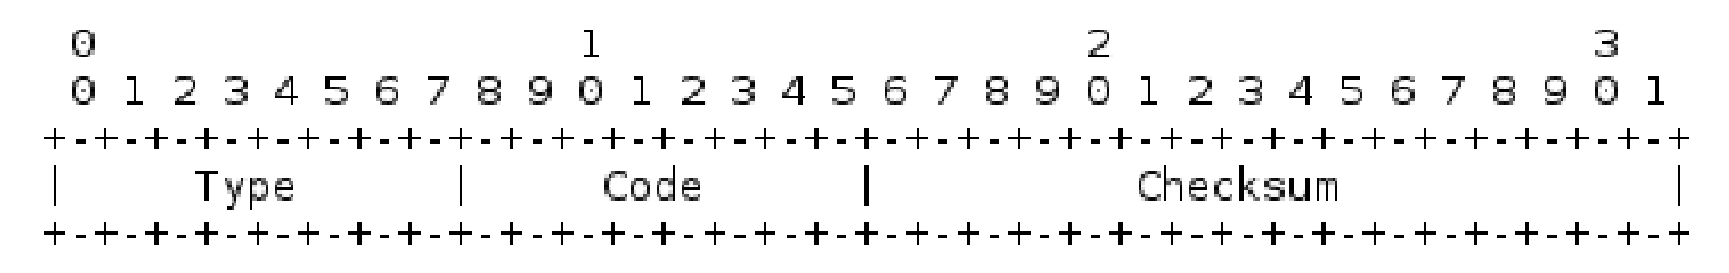
\includegraphics[width=15cm]{./pics/header.eps}
\\Le premier champ est celui de type. Il permet, premièrement, de donner le type du paquet et de l'information à transmettre, et deuxièmement de préciser la nature des champs qui vont suivres. En effet, comme vu plus haut, les messages contiennent des champs différents selon le type du message ICMP.
\\Le deuxième champ est le code. Il permet de subdiviser le type en donnant des détails plus précis.
\\Enfin le troisième champ est la somme de contrôle (checksum)//TODO(plage de controle).
\\Commençons avec les messages qui possèdent l'ensemble de champs le plus simple.

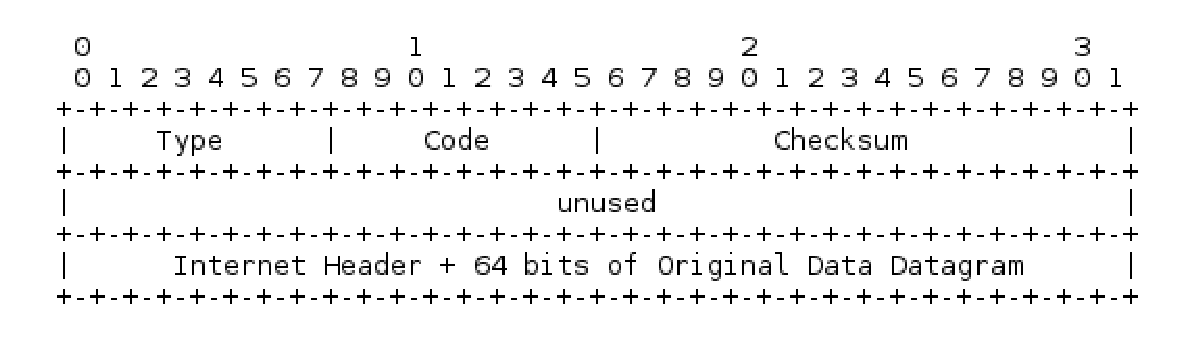
\includegraphics[width=15cm]{./pics/header1.eps}

\\Les messages qui utilisent cette organisation sont les messages de type 3, 4 et 11.

\subsubsection{Message de type 3: Unreachable Destination}
Les messages de type 3 sont émis lorsqu'un paquet n'a pas réussi à joindre la destination (Unreachable destination). Cette erreur peux être dut à plusieurs facteurs, et les codes permettent de préciser pourquoi le paquet n'a pas pu rejoindre sa destination.
\paragraph{Code 0}

\subsubsection{Message de type 4:}

\subsubsection{Message de type 11: Time Exceeded}
Ces messages sont envoyés lorsque le TTL d'un paquet à atteind 0. Une autre utilisation des ces messages est lorsque que le temps de ré-assemblage des fragments d'un paquet est dépassé. Ces deux cas sont distingé par le code. Ces messages ont pour destinataire l'hôte qui à envoyé le paquet qui à provoqué l'erreur.//TODO(vérifier)
Le champ Internet header contient l'entête du paquet qui a été supprimé plus les 64 bits suivant celui-ci. Cela permet à l'émetteur de retrouver quel paquet à été supprimé.
\paragraph{Code 0:}
Le code 0 est utilisé pour indiquer que le TTL du paquet posant problème est arrivé à 0. Lorsque le TTL d'un paquet arrive à 0, celui-ci est supprimer et un message ICMP de type 11 et de code 0 est envoyer par le routeur qui à détécté le problème. Cela permet principalement d'éviter qu'un paquet sans dans une boucle et qu'il soit rélayé à l'infini.
\paragraph{Code 1:}
Le code 1 est quant à lui utilisé pour indiquer //TODO


\subsubsection{Message de type 5:}
Les message de type 5 utilisent les entêtes ci-dessous et servent à faire de la redirection. En effet, lorsqu'un routeur détecte que le prochain routeur dans lequel va transiter le paquet se trouve dans le même réseau que l'émetteur de ce paquet, il va envoyer un message ICMP pour avertir cet hôte (et/ou le réseau) qu'il existe un chemin plus court en envoyant directement les paquets vers le prochain routeur. Ce message ICMP va avoir pour effet de modifier la table de routage interne à l'émetteur (et/ou des hôtes connecté au réseau). Concernant le paquet que le premier routeur à reçu, il va le transmettre vers sa destination.

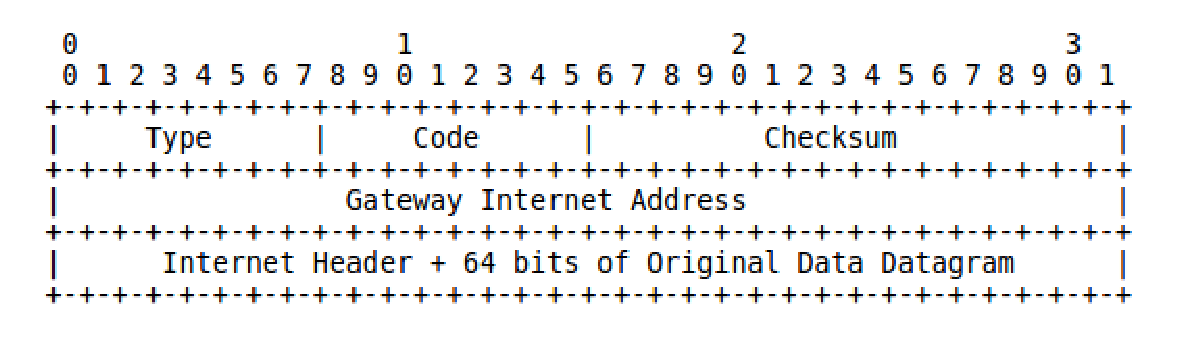
\includegraphics[width=15cm]{./pics/header2.eps}

\\
Le champ Gateway Internet Address contient la l'adresse du routeur auquel il faut faire transiter le traffique directement pour avoir un chemin de routage plus court.
Le champ Internet Header contient toujours l'entête du message ayant porvoqué l'envoie du message ICMP plus les 64 bits suivant l'entête. Cela permet à (aux) hôte(s) de pouvoir modifier leur table de routage en fonction la destination que cherchait à atteindre le paquet.
\paragraph{Code 0}
Ce code indique que la redirection est adresser à tout le réseau de l'émetteur du paquet.
\paragraph{Code 1}
Ce code indique que la redirection est adresser à l'émetteur du paquet.
\paragraph{Code 2}
Ce code indique que la redirection est adresser à tout le réseau de l'émetteur du paquet et aux services(//TODO(préciser)).
\paragraph{Code 3}
Ce code indique que la redirection est adresser à l'émetteur du paquet(//TODO(préciser)).

\\
\\
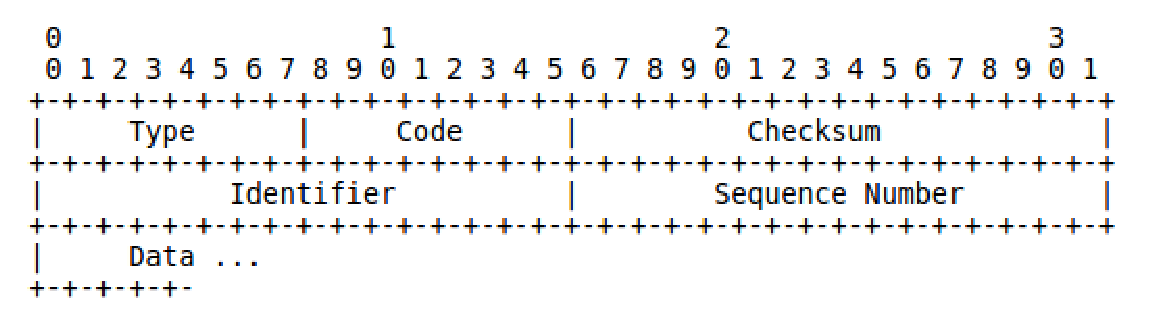
\includegraphics[width=15cm]{./pics/header3.eps}
\\

\subsubsection{Message de type 8 et 0:}
Les messages de type 8 et 0 servent à faire des envoies et des renvoies d'information. Ils utilisent pour cela l'entête ci-dessus. Les messages de type 8 font des envoies d'informations, appelé echo request. Tandis que les messages de type 0 sont envoyés en réponse aux echo request et renvoie les informations reçus de ceux-ci; ils sont appelés echo reply. Etant donnée que les echo reply sont des réponses aux echo request, l'adresse destination des echo reply est l'adresse source des echo request. Ces deux messages peuvent envoyés et reçu aussi bien par un hôte que par un routeur. Ce sont notamment les message envoyés par la commande {\it ping} qui permet de vérifier si l'on peux communiquer avec un hôte ou un routeur.
Les champs Identifier et Sequence Number aide l'émetteur de l'echo request à associer les echos request qu'il à envoyés avec les echos reply qu'il à reçus.
//TODO(qui a t-il dans data?)
\subsection{IGMP}


\subsection{DHCP}
\footnote{RFC 2131: https://tools.ietf.org/html/rfc2131}
Le protocole DHCP (Dynamic Host Configuration Protocol) sert à l'autoconfiguration des interfaces. Plus précisement, il  permet d'attribuer une adresse IP à une interface et de lui faire parvenir d'autres information essentielle pour le fonctionnement de l'interface sur le réseau.
Voyons comment une interface peut ce configurer aurpès d'un serveur DHCP.

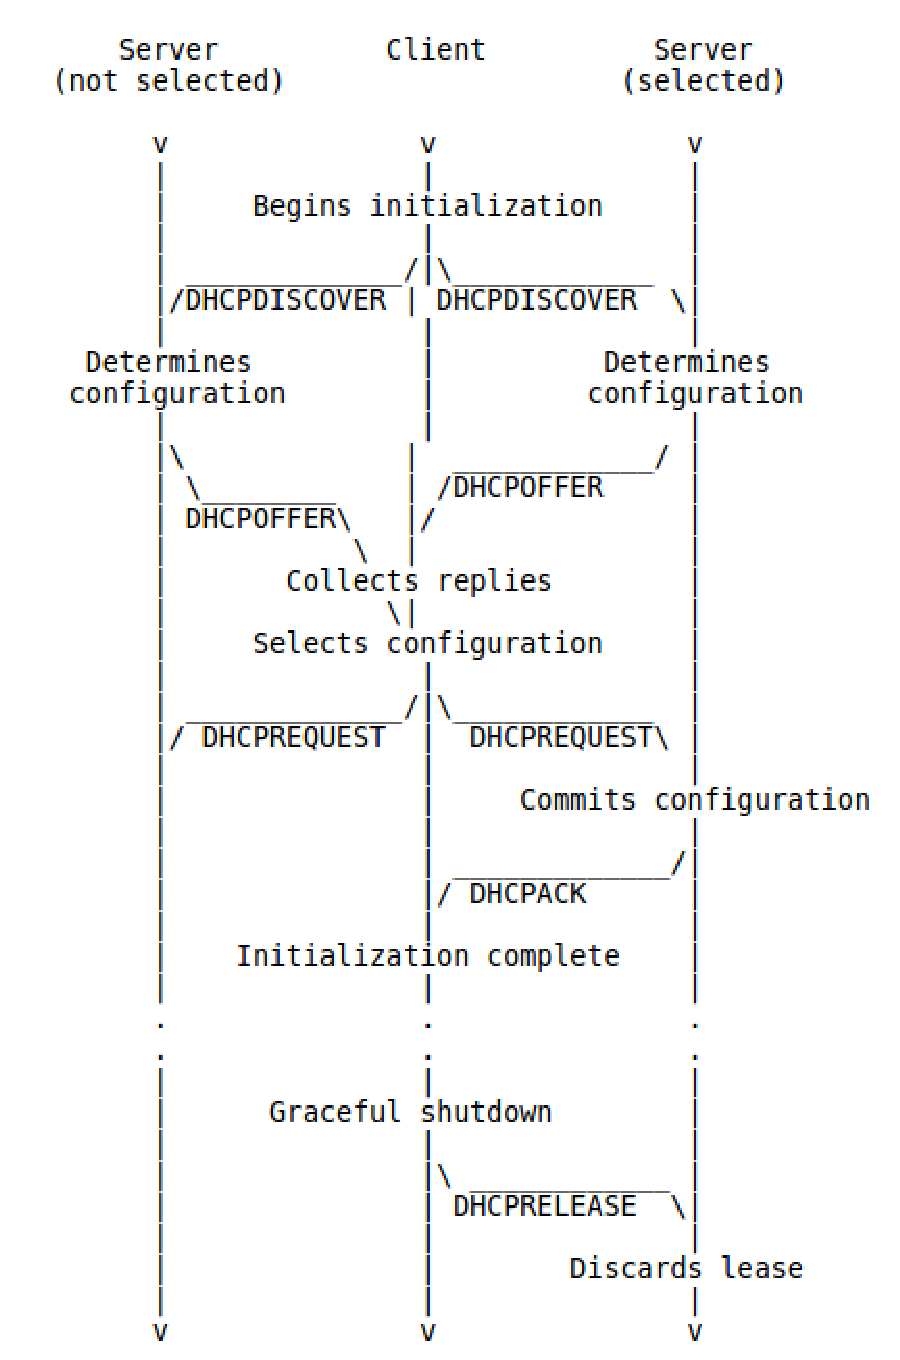
\includegraphics[width=6cm]{./pics/timeline_dhcp.eps}
\\
Lorsqu'une interface, qui n'a pas d'adresse IP, souhaite en recevoir une, elle va emettre un message DHCPDISCOVER en broadcast sur son réseau. Des agents DHCP peuvent faire passer ce message DHCP sur un autre réseau si le serveur DHCP (qui distribue les adresses) ne se trouve pas sur le même réseau que l'hôte qui fait la demande. L'hote va utiliser comme adresse IP 0.0.0.0.
\\Etant donnée que le message est envoyé en broadcast, tout les hôtes sur le réseau vont recevoir le message, et en particulier le ou les serveurs DHCP qui pourraient s'y trouver. Si cela est le cas, ceux-ci vont répondre avec un DHCPOFFER. Ce message contient entre autre l'adresse IP proposé pour le client souhaitant se configurer, ainsi que le masque de sous-réseau de l'adresse. A ce moment là l'adresse n'est pas encore attribuer et réservé pour l'hôte étant donnée qu'il peux refuser l'offre et accepter l'offre d'un autre serveur. Si jamais l'hôte ne reçoit aucun DHCPOFFER, il va ré-émettre un DHCPDISCOVERY. Si il reçoit un ou plusieurs DHCPOFFER, l'hôte va devoir choisir une configuration qui lui est proposé. Une fois ce choix fait, il va informé les serveurs DHCP de son choix à l'aide d'un message DHCPREQUEST émis en broadcast. Ce message va contenir l'identifiant du serveur DHCP retenu ainsi que la configuration souhaité par l'hôte (adresse IP et masque de sous-réseau). Ce message peut être interprété de deux manières différentes selon le serveur:
\item- si ce n'est pas le serveur retenu, il considère le message comme une déclinaison de l'offre.
\item- si c'est le serveur retenu, il va sortir l'adresse attribué l'hôte de la plage d'adresse libre pour ne plus l'attribuer à un autre hôte. Il va ensuite émmetre un message DHCPACK contenant la configuration effective de l'hôte avec notemment: l'adresse IP, le masque de sous-réseau, la durée du bail, l'adresse de la passerelle par défaut et l'adresse du serveur DNS.
Si pour quelque raisons le serveur n'est pas capable d'attribuer l'adresse proposé dans l'offre (par exemple si l'adresse à été attribuer entre temps), le serveur emet un DHCPNAK pour avertir l'hôte que l'adresse n'est plus disponible. L'hôte devra alors recommencer la procédure pour obtenir une adresse IP.
\\Enfin si le serveur ne reçoit pas de message DHCPREQUEST, la procédure s'arrêtrra à ce moment et l'adresse n'étant pas encore attribuer à l'hôte elle reste disponible pour être attribuer à d'autre hôte.
Arrive la dernière étape. Si le client reçois un message DHCPACK, il peux prendre en compte la configuration (adresse IP, masque de sous-réseau, DNS, passerelle par défaut et durée de bail). Il va effectuer une dernière vérification pour s'assurer que l'adresse qui lui à été attribué est bien unique sur le réseau pour éviter d'avoir deux hôte avec la même adresse. Il va pour cela utilisé le protocole ARP et la méthode de vérification vu plus haut. Si jamais l'adresse est déjà utilisé par un autre hôte, il va envoyer un message DHCPDECLINE au serveur DHCP pour lui indiquer qu'il n'utilisera pas la configuration proposé par celui-ci, et il va recommencer la procédure pour pouvoir obtenir une nouvelle configuration.
\\Si jamais l'adresse proposé par le serveur est unique sur le réseau, la configuration est terminé et l'hôte peut utiliser l'adresse (durant la durée du bail de celle-ci).
Dernier cas possible, si jamais le l'hôte ne reçoit pas de DHCPACK ou de DHCPNAK, il va réemettre le message DHCPREQUEST pour esperer recevoir une réponse du serveur.

//TODO algo de retransmission
//TODO fonctionnement agent relais dhcp
//client peut renoncer à son bail
//identification des message faisant partit d'un meme echange avec client identifier, server identifier
//TODO fonctionnement bail

L'hôte est donc configuré et peut utiliser son adresse. Cependant, il ne peut l'utiliser que durant la durée de son bail. Une fois le bail expiré, l'hôte ne peux plus utiliser son adresse. Lorsque l'hôte à reçu le message DHCPACK du serveur, celui-ci lui a transsmis la durée du bail. De cette durée, l'hôte va en extraire deux temps noté T1 et T2. T1 correspond à la moitié de la durée du bail et T2 à 0.875 la durée du bail. Ces temps sont exprimé de manière relatif étant donnée que les horloges du serveur et de l'hôte ne sont pas synchronisées.
Une fois que l'hôte à atteind le temps T1, il va chercher à contacter le serveur qui lui à attribué sa configuration avec un message DHCPREQUEST pour étendre la durée de son bail. Ce message est émis de manière unicast. A ce moment l'hôte est entré en état RENEWING. Si l'hôte reçoit un message DHCPACK du serveur lui accordant un prolongement de la durée de son bail, alors il va sommer le temps qu'il avait insérer dans le DHCPREQUEST avec la durée accordé par le serveur et qui se trouve dans le message DHCPACK. L'hôte retourne dans l'état BOUND. Cependant l'hôte n'est pas obligé d'attendre T1 pour pouvoir étendre son bail.
Si jamais l'hôte ne reçoit pas de reponse DHCPACK avant l'arrivé de T2, il passe en état REBINDING. A ce moment il va émettre un DHCPREQUEST en broadcast pour espérer pourvoir étendre son bail auprès de n'importe quel serveur DHCP. Pour parer aux eventuels cas de perte de DHCPREQUEST, l'hôte va renvoyer un message une fois la moitié de la durée entre T1 et T2 passé, en état RENEWING; et une fois la moitié de la durée entre T2 et la fin du baille , en état REBINDING(et avec un minimum de temps de 60 secondes).
Si malgré tout, la durée du bail venait à expirer, alors l'hôte ne possèderait plus de configuration réseau et ne pourrait plus communiquer avec d'autre hôtes. Il rentre alors en état INIT; il doit alors recommencer la procédure pour obtenir une adresse configuration.

Cependant,dans ce cas comme dans d'autre, l'hôte peut ré-utiliser une configuration précédement utilisée. Cela permet de raccourcir la négociation entre l'hôte et le serveur DHCP. L'hôte va directement commencé la négociation en faisant un DHCPREQUEST en broadcast et contenant la configuration qu'il souhaite ré-utiliser. Le serveur concerné par l'attribution antérieur de la configuration va donc accepter la demande de l'hôte à l'aide d'un DHCPACK ou la refuser, si la demande n'est pas correct ou si l'adresse est utilisé par un autre hôte, à l'aide d'un DHCPNAK.
Cette négociation se fait de manière similaire qu'un négocation complète, elle a juste été raccourci en enlevant quelque étape non indispensable.

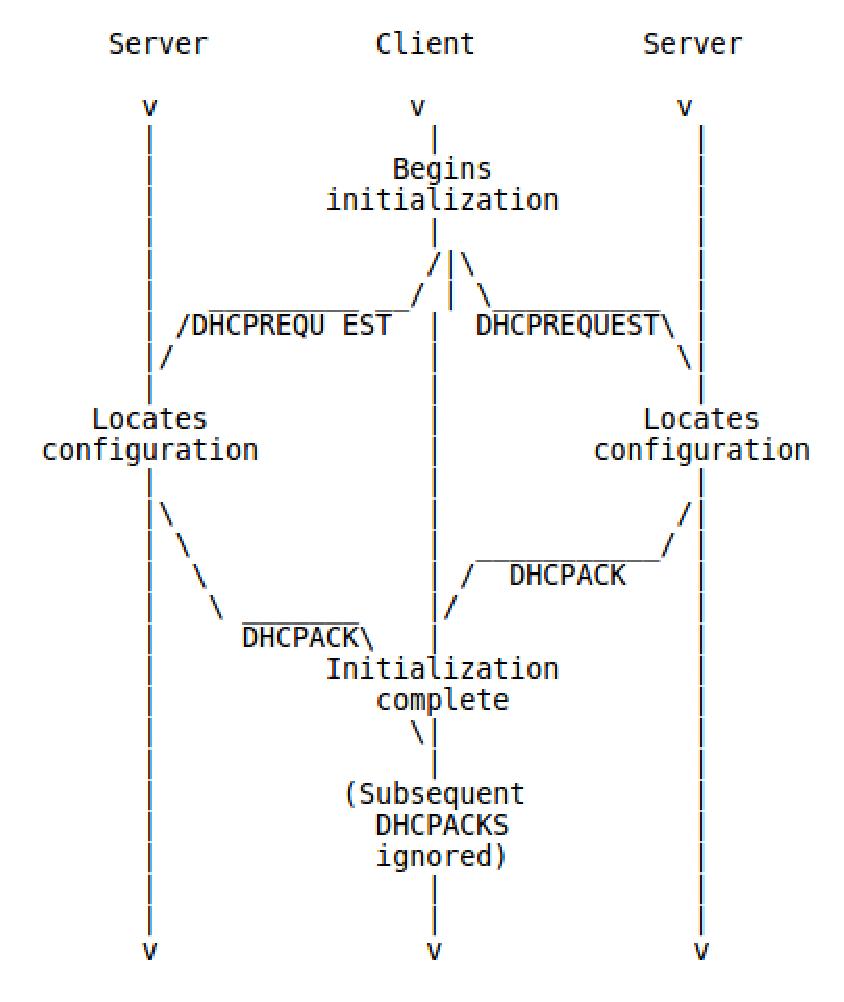
\includegraphics[width=6cm]{./pics/timeline_dhcp_reuse_add.eps}
